\section{Grappa Overview}

\begin{figure}[t]
\begin{center}
  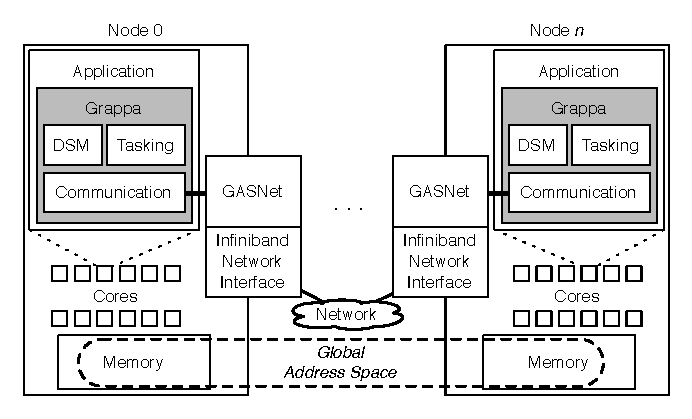
\includegraphics[width=0.95\columnwidth]{figs/system-overview}
\begin{minipage}{0.95\columnwidth}
  \caption{\label{fig:grappa} Grappa system overview}
\end{minipage}
\vspace{-3ex}
\end{center}
\end{figure}


Grappa (Figure~\ref{fig:grappa}) has three main software components:
\begin{description}

\item [Tasking system.] Our tasking system supports lightweight
multithreading to tolerate communication latency and global distributed
workstealing (i.e., tasks can be stolen from any node in the system), which
provides automated load balancing.

\item[Distributed shared memory.] Our DSM system provides support for
fine-grain access to data anywhere in the system. It supports synchronization
operations on global data, explicit local caching of any memory in the system,
and support for operation on remote data (delegating operations to home node).
By tight integration with the tasking system and the
communication layer, our DSM system offers high aggregate random
access bandwidth for accessing remote data.

\item[Communication layer.] As discussed earlier, modern commodity networks
support high bandwidth only for large messages. Since irregular applications
tend to need frequent communication of small requests, the main goal of our
communication layer is to aggregate small messages into large ones to better
exploit what the network can offer. It is largely invisible to the application
programmer.

% software developer but helps to improve network performance when applications read and write only small pieces of data.

\end{description}

% \paragraph{Exploiting Latency Tolerance} As we will show later, Grappa can tolerate latencies way beyond that of the network. Therefore, Grappa can afford to \emph{trade latency for throughput}: by {\em increasing} latency in key components of the system we are able to increase our aggregate random access bandwidth (by delaying and aggregating messages), our synchronization bandwidth (by delegating operations to remote nodes), and our ability to improve load imbalance (work stealing increases latency).

% \TODO{check to see we actually explain these three somewhere.  Ie, that aggregating increases throughput and latency, that delegating synchronization increases the rate and the latency at which we can eg atomically increment, and that stealing work increases the latency of some tasks (eg when their data is largely at the originating node) but provides greater throughput overall.}

In the next three sections we describe both Grappa's main capabilities and how they are implemented.

